\documentclass{standalone}
\usepackage{pgfplots}
\pgfplotsset{compat=1.17}
\usetikzlibrary{arrows}
\tikzset{>=latex'}
\begin{document}
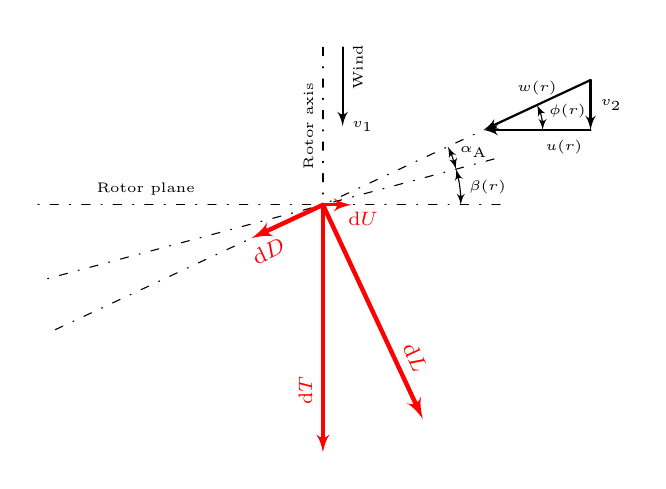
\begin{tikzpicture}[scale=5,line cap=round]

\path [use as bounding box,red] (-0.5,-0.65) rectangle (1.05,0.45);

\begin{scope}[rotate around={180:(.25,0)}]

% Airfoil
\begin{scope}[rotate around={15:(.25,0)}]
\filldraw[draw=blue,fill=blue!10!white] plot file{naca643618.dat} -- cycle;
\draw[loosely dash dot] (-.2,0) -- (1,0);
\end{scope}

%Rotor plane and axis and wind v_1
\draw[loosely dash dot] (-.2,0) -- (1,0) node[above,near end]{\tiny{Rotor plane}};
\draw[<->] (-.1,0) arc (180:195:.35) node[right,midway]{\tiny{$\beta(r)$}};

\draw[loosely dash dot] (.25,-.4) -- (.25,0) node[sloped,above,midway]{\tiny{Rotor axis}};
\draw[thick,->] (.2,-.4) -- (.2,-.2) node[sloped,below,near start]{\tiny{Wind}};
\draw (.2,-.4) (.2,-.2) node[right]{\tiny{$v_1$}};

% Trinagle and forces
\begin{scope}[rotate around={25:(.25,0)}]
    \draw[loosely dash dot] (1,0) -- (-.2,0);
    \draw[<->] (-.35,0) arc (180:155:.15) node[right,near start]{\tiny{$\phi(r)$}};
    \draw[<->] (-.1,0) arc (180:170:.35) node[right,near start]{\tiny{$\alpha_{\textnormal{A}}$}};
    \draw[->,thick] (-.5,0) -- (-.2,0) node[above,midway]{\tiny{$w(r)$}};
    \draw[->, thick, rotate around={-25:(-.5,0)}] (-.5,0) -- (-.5,.12679) node[right,midway]{\tiny{$v_2$}};
    \draw[<-, thick, rotate around={-25:(-.2,0)}] (-.2,0) -- (-.47189,0) node[below,near end]{\tiny{$u(r)$}};
    \begin{scope}[red,ultra thick]
        \draw[->] (.25,0) -- (.25,.6) node[rotate=-65,above,near end]{\footnotesize{d$L$}};
        \draw[->] (.25,0) -- (.45,0) node[below,very near end,rotate=25]{\footnotesize{d$D$}};
    \end{scope}
    \begin{scope}[red,very thick]
        \draw[->,rotate around={-25:(.25,0)}] (.25,0) -- (0.17769,0) node[below=5pt,right=-5pt]{\scriptsize{d$U$}};
        \draw[->,rotate around={-25:(.25,0)}] (.25,0) -- (.25,.62831) node[above,near end,sloped]{\scriptsize{d$T$}};
    \end{scope}
\end{scope}

\end{scope}
\end{tikzpicture}
\end{document}